This chapter provides a high-level overview of the core components of the AirSim architecture. The chapter will look at how the simulator has been adapted for this project, the design decisions made, and the limitations. 

As the project is extending an existing code-base, the design decisions aimed to limit the impact on the existing structure. This was to allow future updates to the master project, to benefit this one as well. Most of the changes to this project were made in Unity, but changes were also made in AirLib and the wrapper to allow for additional APIs. 

\section{AirSim Functional Overview} \label{05:Overview}
Figure~\ref{ADA:Figure:OriginalOverview} shows a simplified overview of the important components in the original AirSim architecture. It is key to understand each of these components, as they are all updated throughout the project. 


The project consists of 4 main components, Unity, which is written in C\# and contains most of the simulator logic, AirLib which is written in C++ and contains the server, the AirLib Wrapper which is written in C++ and acts as a bridge between AirLib and Unity, then finally the code where the user can interact with AirLib through the APIs. As this project is very modular, it gives the user the freedom and flexibility to choose a game engine and input language. 

This section will contain a brief overview of each of the 4 components. This is to better understand the design decisions made in Section~\ref{05:ArchitecturalDesign}.

\begin{figure}[h]
    \centering
    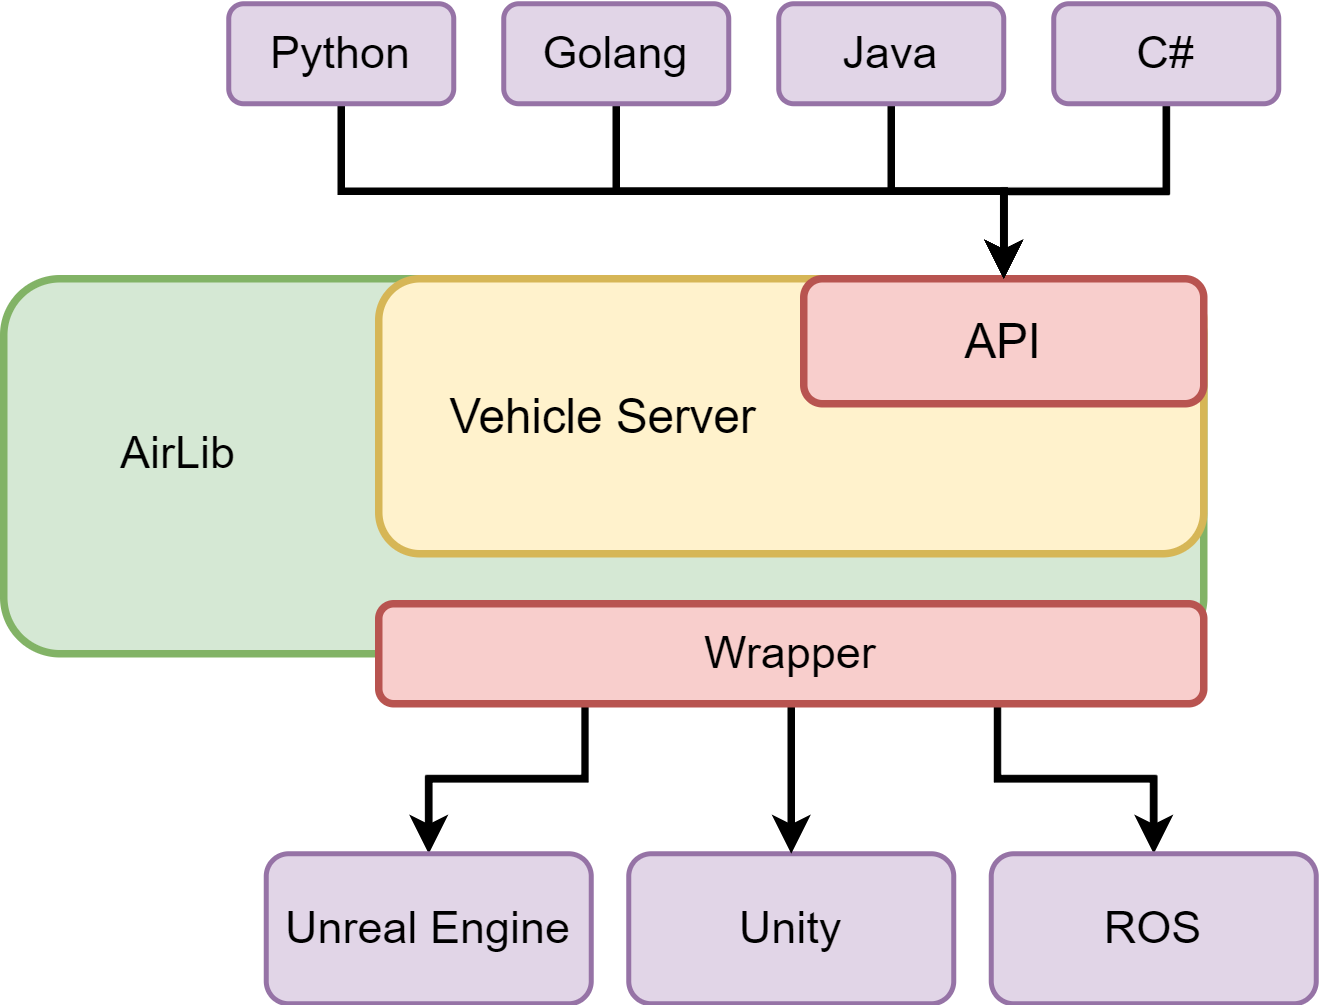
\includegraphics[width=0.5\textwidth]{05_AnalysisAndDesign/Diagrams/OriginalOverview.png}
    \caption{High-level overview of the core components of AirSim used for this project. Only one server exists and all API calls are passed to it.}
    \label{ADA:Figure:OriginalOverview}
\end{figure}


\subsection{AirLib} \label{05:AirLib}
AirLib is the main component of AirSim and where the majority of the code is located \cite{}. This self-contained library consists of four main components. The first one is a physics engine. This component is lightweight and designed to be simple to add new vehicles and drones. The next component is a sensor model. This component contains header-only models for external sensors such as GPS and Barometer. The third component is the vehicle module. Currently, the only model implemented is for PX4 QuadRotor\footnote{\url{https://docs.px4.io/master/en/getting\_started/}}, which is a platform that can be used to control drones. The last component is the control library. This part provides abstract classes for the APIs and implementations for specific platforms. 

This project does not use the physics engine, sensors module and vehicle modules in AirLib. The project is instead using the Unity version of these components. Instead, this project focuses almost solely on extending the control library. On startup, AirLib creates AirLib creates a server using RPCLib\footnote{\url{https://github.com/rpclib/rpclib}} which can interact with the APIs over a TCP channel. The advantage of using RPC is that it allows for a range of different programs as well as being fast and lossless (Section~\ref{05:UIL}). The design decision to move the physics engine and sensors to Unity is further discussed in Section~\ref{05:ArchitecturalDesign}. 

\subsection{AirLib Wrapper}
A wrapper is used for AirLib to communicate with Unity. Using a wrapper allows for a variety of different game engines as well as other physical systems such as ROS. This makes AirSim more modular, which again can increase the extensibility of the program. The wrapper will implement the interfaces declared in the vehicle module (Section~\ref{05:AirLib}). At startup, Unity will pass function pointers to the wrapper so that later the APIs can call those functions. The wrapper will also create an instance of AirLib which will set up the RPC server. The wrapper also handles the conversion of the data from C\# to C++.

\begin{figure}[h]
    \centering
    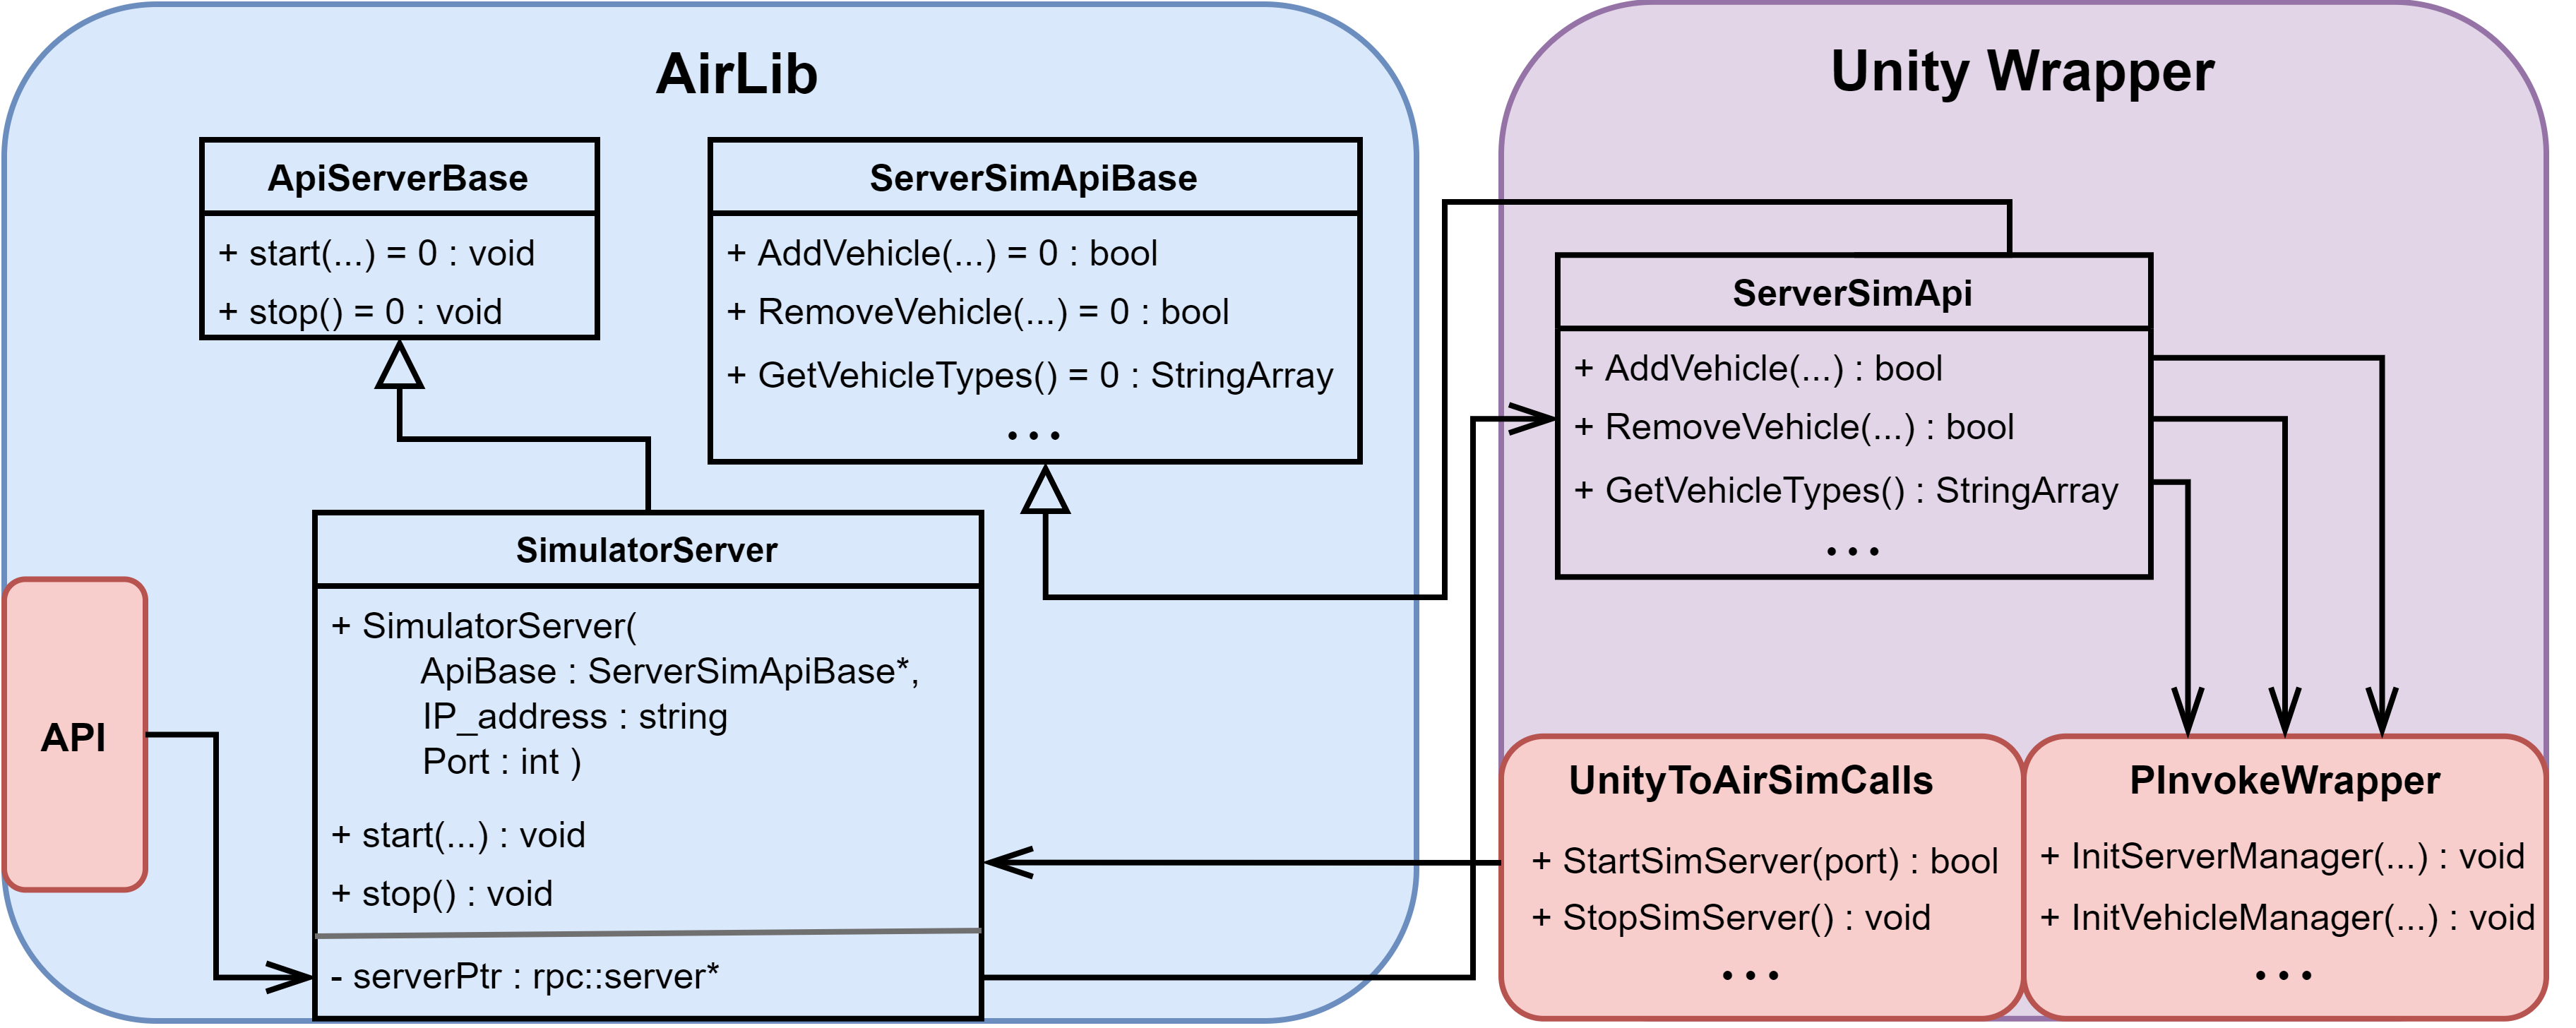
\includegraphics[width=1\textwidth]{05_AnalysisAndDesign/Diagrams/UnityWrapper2.png}
    \caption{A simplified view of how AirLib and the Unity Wrapper link together. UnityToAirSimCalls and PInvokeWrapper are red boxes to illustrate that they are only files containing functions. The other objects are classes. The black arrows show examples of functions calls. The details of how Unity starts the server is left out in this diagram.} \label{05:fig:UnityWrapper}
\end{figure}

Figure \ref{05:fig:UnityWrapper} shows an example of how AirLib links to the Unity Wrapper. AirLib has an interface for the available APIs that are then overridden in the wrapper. These overridden member functions will then access the function pointers initialised at startup by Unity. This is done by having Unity call the InitServerManager with the arguments being the function pointers. As was explained in Section~\ref{05:AirLib}, the API interacts with the server initialised at startup. In this case, the server is stored in the SimulatorServer class and will call functions overridden from the ServerSimApiBase class. Unity can also make calls to the wrapper at runtime. These are done through the UnityToAirSimCalls. The figure shows a slightly simplified for how Unity can start and stop the server. To create the server, the wrapper creates a new instance of the ApiServerBase and initialises it with a pointer to the ServerSimApi. It is clear from this figure that another game engine can easily be used by changing the overridden functions. 


\subsection{AirSim with Unity}
As will be discussed in Section~\ref{05:AD:UEvUnity}, Unity was chosen as the game engine for this project. Unity works as the physics engine and all of the simulator logic is solely done in Unity. One of the disadvantages of using Unity is that it is not thread-safe. This means that the AirSim plugin has to interact with the simulation through shared memory. This will be explained further in the implementation section (Section~\ref{06:airsim}). All of the simulator logic is solely done in Unity.

AirSim works as a plugin for Unity. AirLib and the wrapper are compiled into a single DLL file which can be interacted with through Unity. This allows the user to use all the features in Unity when creating maps and environments. This also makes it easy to set up an AirSim environment as only the DLL and a setup object has to be added to the scene.  


\subsection{User Interaction Layer} \label{05:UIL}
AirSim allows for a variety of different languages to interact with AirLib. This is because the API calls use MessagePack\footnote{\url{https://msgpack.org/}} also known as MsgPack. MsgPack allows for an efficient binary serialisation\footnote{\url{https://github.com/msgpack/msgpack/blob/master/spec.md}}. MessagePack supports over 50 programming languages and environments. These include C\#, Golang, Haskell and others.  For this project, only Python will be used. This is because Python is a flexible language that makes prototyping quick and easy. The existing code for the user interaction layer is already written in Python, so it will be more beneficial to continue with this rather than starting from scratch.

In the Python project, three classes are implementing the APIs for each of the servers. This is to make it clear which type of entity the user is communicating with. It also avoids confusion when passing controls to the simulator, as pedestrian and vehicles use different controls. Python allows for external tools like OpenCV to process the images passed from the Simulator. Figure~\ref{} shows a diffusion map generated by OpenCV using two images created by forward-facing cameras on a car. The diffusion map highlights objects that are shifted more between the two images, i.e. the object has to be closer. 









\section{Architectural Design and Limitations} \label{05:ArchitecturalDesign}
This section will look at some of the architectural decisions made when modifying the existing AirSim design. The section will also look at what limitations were introduced by these decisions. Section~\ref{06:airsim} will go into more detail about how the design decisions were implemented. 


\subsection{Unreal Engine or Unity} \label{05:AD:UEvUnity}
After AirSim was chosen as the simulator, the main decision to be made was which game engine to use. AirSim primarily uses Unreal Engine, but there is also a prototype version using Unity. As mentioned in the background section (Section~\ref{GameEngines}), Unreal Engine has better graphics than Unity. Using Unreal Engine would also mean that the simulator more complete with many more features available such as dynamic weather, more sensors and more APIs. Generally, Unreal Engine also has better performance than Unity\cite{vsmid2017comparison}. The disadvantage of using Unreal Engine is that it makes it harder to rapidly prototype and add new features. This is because the existing code is much more complex. It is also because Unreal Engine is not as simple to use as Unity. In Unity, the simulator can run in debug mode making it possible to update scripts whilst the program is running. This is not possible in Unreal Engine where a small change can take a couple of minutes to compile. 

There are several advantages to using Unity over Unreal Engine. Firstly, Unity's asset store provides a large range of plugins and models that can be used. The key ones that are of interest for this project are the UMA models (Unity Multipurpose Avatar), which can be added to model pedestrians, and the ML-Agents tool kit, which can be used to train reinforcement learning models. Both of these addons will be explained further in the implementation section (Section~\ref{06:airsim}). The second advantage of using Unity is the simplicity of having scripts. This makes debugging simpler as the scripts can be interacted with at runtime. The scripts can also be attached to objects which makes it easy to create several instances of an entity. Another advantage is that as using Unity as the game engine is currently only an experimental version, only the most important features have been implemented. This makes the existing code easier to navigate than the code written for Unreal Engine. This can also be seen as a disadvantage of using Unity. As only a few APIs have been implemented, a lot of work has to be put in to have the same features available in Unity as currently are available in Unreal Engine\footnote{\url{https://microsoft.github.io/AirSim/unity_api_support.html}}. 

Overall using Unity for this project would be more beneficial than using Unreal Engine. Unity allows for rapid prototyping which is more important for this project. Unity's ML-Agent also makes it easier to train reinforcement models for the part of the autonomous system of this project. 

\subsection{Moving logic to Unity}
Section~\ref{05:AirLib} explained how AirLib is split into four parts and that this project would only focus on the vehicle module. AirSim is designed in such a way that software components are easily exchangeable. As can be seen from Figure~\ref{ADA:Figure:OriginalOverview}, ROS, which is a robot operation system, could be used instead of a game engine. AirSim would then be able to model the behaviour of the real robot without needing the game engine. As this project would only focus on the simulation, this was not a feature that was needed. Instead, it was easier to move all the physics calculation to Unity along with other logic such as controlling the vehicles. Making this design decision would make it much easier when adding the pedestrians. Currently, the physics engine in Unity would need a redesign to get something like autonomous wheelchairs and pedestrians to work.

The consequence of this is that the simulation behaviour could differ between the different game engines. AirSim would also not work for pedestrians without the Unity game engine. As this project is only a prototype, the simplification of moving the logic to Unity will still be beneficial. 

% Modularity
\subsection{Dividing the server}
The decision to split the server in AirLib was the main change to the existing design of AirSim. This design change was needed for several reasons. Firstly, how the server is implemented currently, all API calls are single-threaded, which means that one call has to be processed before the next one is handled. This makes the API that captures images slow as it has to wait for one game tick before returning the image. (See Figure~\ref{06:imageCapture} in Section~\ref{06:airsim}). Another reason for doing this was to simplify the code structure. As can be seen from Firgure~\ref{05:SplitServer}, dividing the AirLib server to handle the game state, vehicles and pedestrians separately was a natural split, especially as the pedestrians would introduce a large number of new APIs. This split would make it clear which entity is being controlled and which APIs are available. Also, in the current design, the server only exists if there is a vehicle in the scene. If the vehicle is removed, the server is closed. This also means that there has to be a vehicle in the scene to start the server.  This is not the desired behaviour as a user would want to be able to spawn in and delete both vehicles and pedestrians at any time. 

\begin{figure}[h]
    \centering
    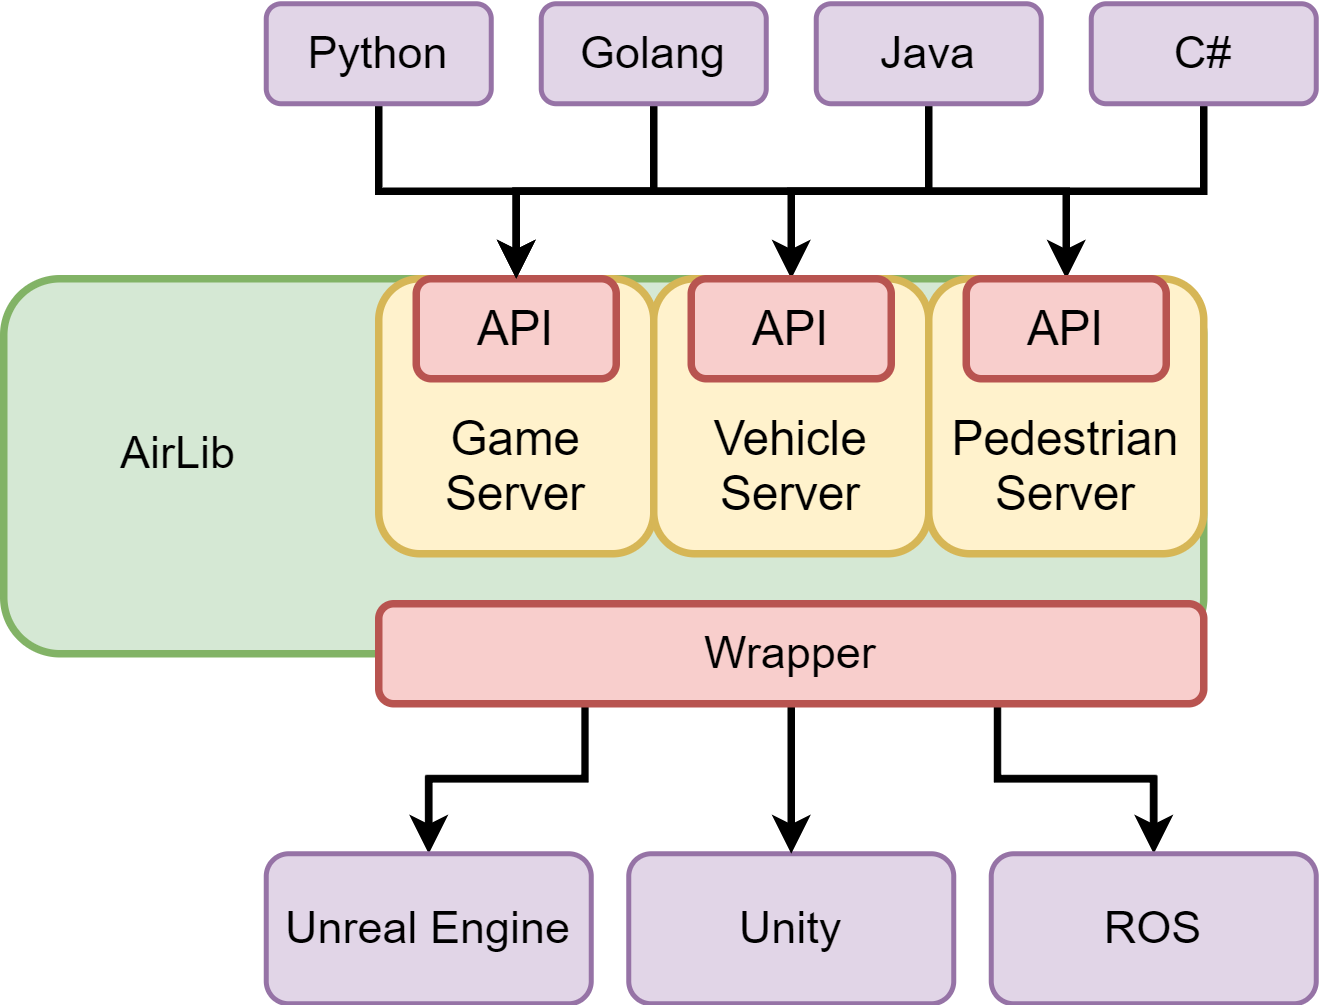
\includegraphics[width=0.5\textwidth]{05_AnalysisAndDesign/Diagrams/UpdatedOverview.png}
    \caption{Separate APIs into several servers on different ports. This makes it easier to expand the APIs and add additional features.}\label{05:SplitServer}
\end{figure}

The division was done by replicating a simplified version of the server creation and then moving the APIs for the game state over to this one. As mentioned in the functional overview (Section~\ref{05:Overview}) AirLib has a lot of features that this project does not need. When replicating the server initialisation, these parts were left out. In Unity, the code was changed in such a way that at startup, the game server will start, and the user can communicate with the server, such as printing, spawning and deleting vehicles and pedestrians, and so on. When the first vehicle is spawned the server vehicle server will start, and when the last is deleted, the server will close. This behaviour is the same for the pedestrians. 

This project benefits in several ways when dividing the server. Firstly, as mentioned above, the server would now start running at startup. This means that users can control the game state without vehicles having to be in the scene. Secondly, dividing the APIs makes the code more readable. Originally it is difficult to see if an API call acts on the server or the vehicle. Another benefit of the split is that the game server can communicate instantly with the server instead of having to wait for the other calls to the vehicle server to finish. Finally, with the current implementation, it would be easy to open up a separate server for every vehicle. This could be beneficial as separate scripts could run a specific vehicle. This change is now possible as the code is designed in such a way that it can start a new server on request. 

However, there are several limitations and disadvantages to this new approach. Firstly, if too many servers are launched the overhead will be too big and the performance would decrease. Currently, this is not an issue with only three servers, but with one server per entity, this could be slow. Secondly, if for example, a developer wants to use different means of communication for the APIs, rather than RPC, this would require several changes in multiple files. Finally, as this is a major change to the existing AirSim, pulling new features from the master repository will no longer be straightforward. 

Overall the benefits still outweigh the disadvantages. As having multiple entities in the scene at once is a key part of this project, separating the APIs relating to the game from the APIs relating to the vehicle allows for this. This also works as a proof of concept if performance becomes an issue and a server per entity becomes needed. 


%Why was this needed.
% •	Server was only single threaded
% •	This meant slow especially when getting images
% •	Pedestrian controls were different. Make it easier to distinguish between the two.
% •	Separate server controlling APIs
% •	Limit the number of API calls going to one serverS
% How was this done
% •	Extract Server APIs from the existing vehicle server
% •	Create Pedestrian API server from scratch. 
% How does it improve things	
% •	Makes it more readable as everything is not in one big class.
% •	Makes it possible to control pedestrians and vehicles from different scripts
% •	A simple modification can be made to set up even more servers, for example one per entity.
% •	If multiple servers was created they would still communicate in the same way with Unity, so every instance could still talk to every entity. 
% •	Simulator at startup
% What does it break/limitations
% •	If for example wanted to use different communications means than RPC, this would require changes in several files. 
% •	In some ways not as easy to navigate as all the code is not in one place. 
% •	Increased server overhead. (Not much for 3, but if there were over 100 this could be a problem. 
% •	As this is a major change to AirLib, future updates to AirSim will not be incorporated automatically. 


%\subsection{Simplifications}
%\section{Architectural Limitations}

